\newpage


\section{Case Studies}
\label{sec:case-studies}

While the handcrafted NNs yielded relatively acceptable results we ask ourselves: how do other, well known,
model perform with such a trivial task? \\To answer this question two "case studies" were selected: Xception and VGG16.

\subsection{Xception}
\label{subsec:xception}

The Xception\cite{chollet2017xception} model was developed by Google and is an evolution of the Inception model presented
during the ImageNet Recognition Challenge of 2012.

The Inception family of models are defined by a low count of parameters compared to competitors but, what makes
\textit{Xception} special, is that the use of depthwise separable convolutions throughout the network\cite{understandingdeepwise}. % todo valuta se toglierlo
\begin{figure}[h]
    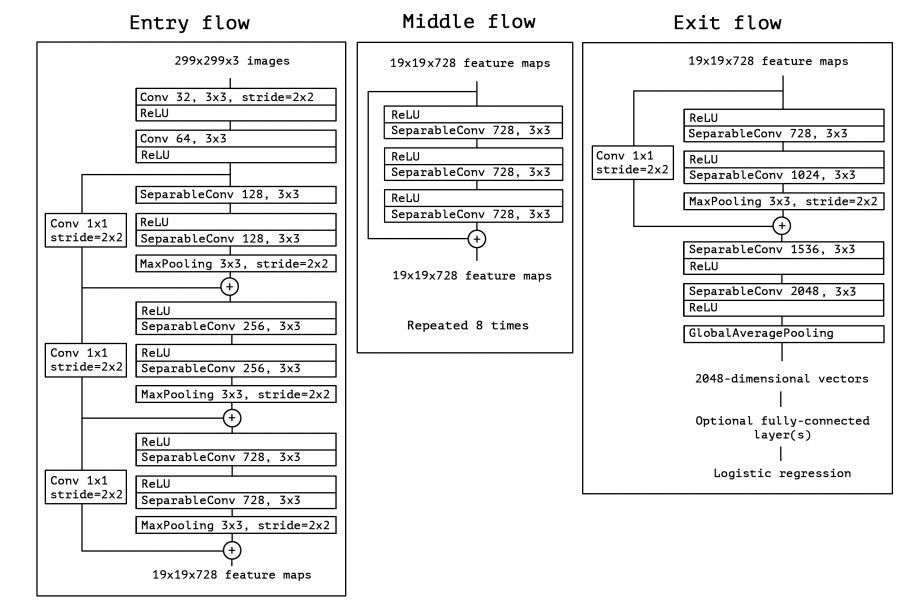
\includegraphics[scale=0.4]{imgs/xception-arch}
    \caption{
        Xception is made of a total of 71 layers.\\
        \textit{Image by the author of the original paper Francois Chollet\cite{chollet2017xception}}
    % todo ref

    }\label{fig:figure}
\end{figure}

\subsubsection{Xception applied to Muffin vs Chihuahuas}
\label{subsubsec:xception}

To measure the performance of Xception on the Muffin vs Chihuahuas task we first see the pretrained model in action
to later fine tune it on our dataset.

\paragraph{Pretrained Model} The pretrained model used in the project for the evaluations was trained on the\textit{Imagenet} dataset.
The dataset does not provide a label "muffin" so it was mapped to "bakery"(415) which for our intent is close enough.
Predictions might not include either bakery or chihuahua as there are other classes, in this case we consider them as misclassifications.

When running the network on the test set the performance was low.
It only correctly classified 67.65\% of the samples.
This was to be expected as the classifier is both untrained on muffins and has more labels that might actually fit the given image.
We expect the model to work better once fine-tuned.

\begin{figure}
    \centering

    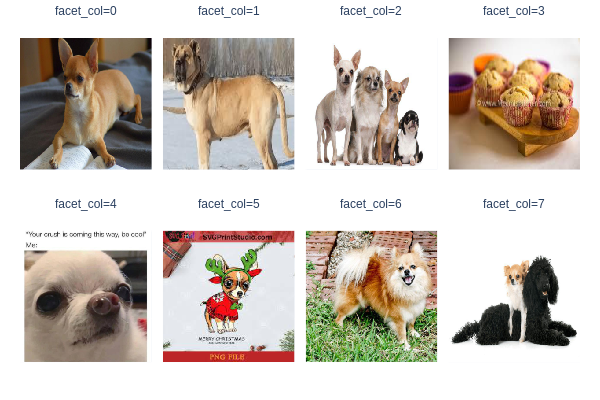
\includegraphics[scale=0.5]{/home/jacopo/PycharmProjects/muffin-stat-project/report/imgs/7_xception_test_images}
    \begin{tabular}{ | c | c | c | }
        \hline
        facet\_id & $y$       & $\hat{y}$                                                \\
        \hline\hline
        0         & chihuahua & ['Chihuahua', 'toy\_terrier', 'miniature\_pinscher']     \\
        \hline
        1         & chihuahua & ['bull\_mastiff', 'bloodhound', 'Great\_Dane']           \\
        \hline
        2         & chihuahua & ['Chihuahua', 'toy\_terrier', 'Mexican\_hairless']       \\
        \hline
        3         & muffin    & ['French\_loaf', 'tray', 'hamper']                       \\
        \hline
        4         & chihuahua & ['Chihuahua', 'Pomeranian', 'papillon']                  \\
        \hline
        5         & chihuahua & ['envelope', 'packet', 'handkerchief']                   \\
        \hline
        6         & chihuahua & ['Pomeranian', 'keeshond', 'Pekinese']                   \\
        \hline
        7         & chihuahua & ['standard\_poodle', 'toy\_poodle', 'miniature\_poodle'] \\
        \hline
    \end{tabular}


    \caption{Some images and relative predictions of \textit{Xception} on our dataset.\\
    Interestingly for facets 1 and 6 the prediction, while misclassified by our considerations, is actually correct
    as the image in the dataset is not really a chihuahua.
    }
    \label{fig:7_xception_test}
\end{figure}


% todo imggine risultati

\paragraph{Fine-tuned Model}
In order to fine tune the model we have to define a new one that wraps around Xception.
The model has to use the pre-processing on data used by Xception as requested by the keras documentation.
It is also necessary to output a single prediction value instead of the previous 1000 classes.

During the training process, which often takes very little time,  we freeze the network to avoid destroying information
already built by the previous training process and only work up on the last layer of the \textit{Xception}%\ref{fig:figurexception}.
%immagine modello
%\begin{figure}[h]

%    \centering
%    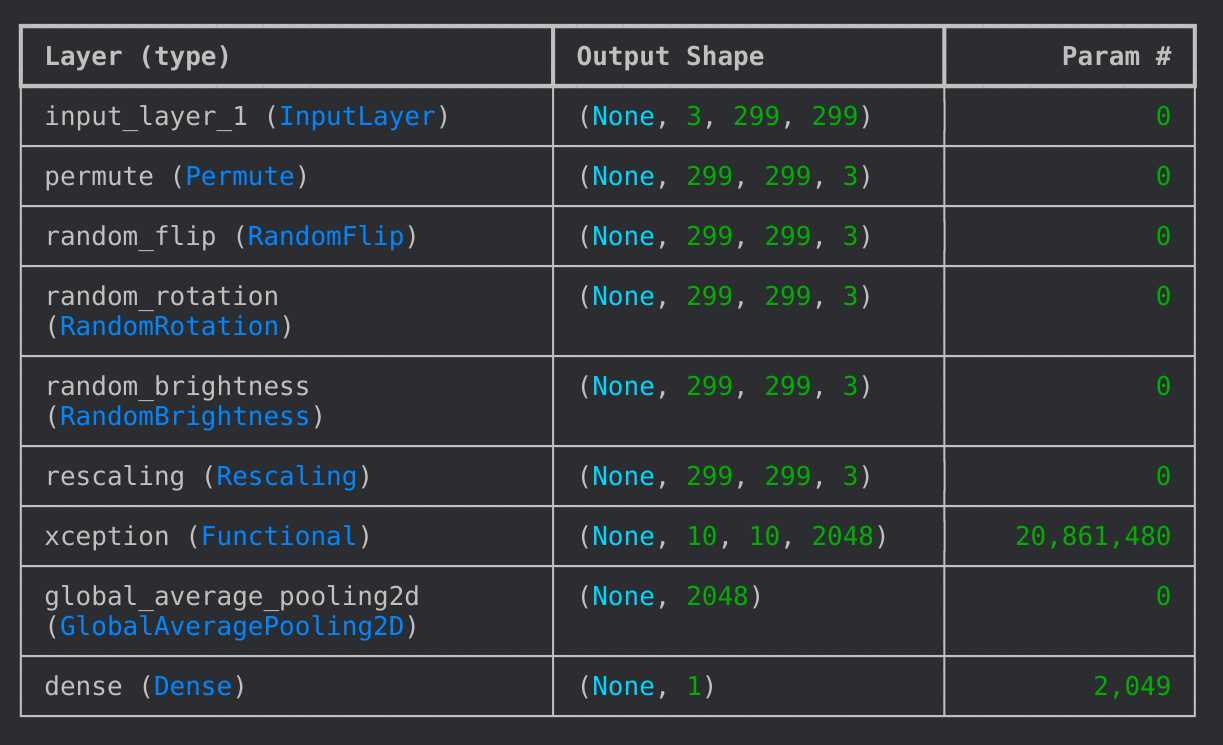
\includegraphics[scale=0.2]{/home/jacopo/PycharmProjects/muffin-stat-project/report/imgs/struct_xception_custom}
%    \caption{
%        Before calling \textit{Xception} the model preprocesses the data with the same augmentation procedure we defined for the other
%        networks of the project. It then also rescales the images to meet the requirement for \textit{Xception}.
%        At the top of the model we have now a single dense neuron layer that will return the classification output.
%    }\label{fig:figurexception}
%\end{figure}

The K-fold CV estimates results lead to a better model than the previously built ones as shown in the Table \ref{tab:kfoldxception}.
The final trained model has has $acc=99.16\%$ and $l_{0-1}=00.84$ which is consistent with the expected values.

\begin{table}
    \centering
    \begin{tabular}{ | c | c | c | }
        \hline
        $k$ & $accuracy$ & $l_{0-1}$ \\
        \hline\hline
        0   & 0.9983     & 0.0017    \\
        \hline
        1   & 0.9916     & 0.0084    \\
        \hline
        2   & 0.9932     & 0.0068    \\
        \hline
        3   & 0.9975     & 0.0025    \\
        \hline
        4   & 0.9940     & 0.0059    \\
        \hline
        \hline
        avg & 0.9949     & 0.0051    \\
        \hline
    \end{tabular}
    \quad
    \begin{tabular}{| c | c | c |}
        \hline
        $k$ & $accuracy$ & $l_{0-1}$ \\
        \hline\hline
        0   & 0.9958     & 0.0118    \\
        \hline
        1   & 0.9916     & 0.0084    \\
        \hline
        2   & 0.9949     & 0.0051    \\
        \hline
        3   & 0.9873     & 0.0127    \\
        \hline
        4   & 0.9907     & 0.0093    \\
        \hline
        \hline
        avg & 0.9905     & 0.0095    \\
        \hline
    \end{tabular}
    \caption{
        Left the \textit{Xception K-fold estimates}, right the \textit{VGG-16} ones.

    }
    \label{tab:kfoldxception}
\end{table}

\subsubsection{Vgg16}\label{subsubsec:vgg16}
Developed by Visual Geometry Group (VGG) at the University of Oxford the VGG-16\cite{simonyan2015deep} is a deep CNN model that
was proposed for the ImageNet Large Scale Visual Recognition Challenge (ILSVRC) in 2014 where it achieved top results in object detection and image classification.

\begin{figure}[h]
    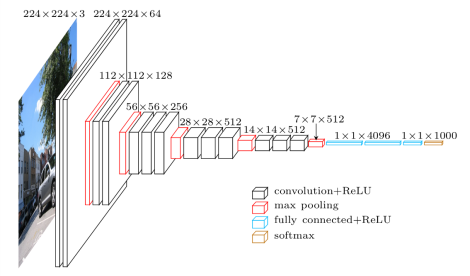
\includegraphics[scale=0.7]{imgs/vgg_arch}
    \caption{
        The VGG-16 model is characterized by 13 convolutionakl layers among which at times a max pooling layer has been placed.
        After those layers the network is closed by 3 fully connected layers with a final softmax classifier.
        \textit{Image by Davi Frossari (https://www.cs.toronto.edu/~frossard/about/)}
    }\label{fig:vgg16}
\end{figure}

Compared to Xception this model has more parameters

\subsubsection{VGG-16 applied to Muffin vs Chihuahuas}
The ideas we applied on Xception and the general methodology (\ref{subsubsec:xception}) are analogous to the ones
applied to \textit{VGG-16}.


\paragraph{Pretrained Model}
As for \textit{Xception}, our used instance model of \textit{VGG-16} was trained on Imagenet.
When running the network on the test set we had poor performance as for the other analized model.
It only correctly classified 57.01\% of the samples, yielding a worse performance than \textit{Xception}.

\paragraph{Fine-tuned Model}
The fine tuning process on the \textit{VGG-16} uses its dedicated
pre-processing function on the data. After a short training period
we ran the K-fold CV estimates which are reported in Table \ref{tab:kfoldxception} which is in line
with the final model having $acc=99.16\%$ and $l_{0-1}=0.084$.
Overall the performance of the classifier is on pair with the one of \textit{Xception}
with one drawback being: it has more parameters. So, from a practical standpoint,
\textit{Xception} could be preferable as the two models is not that far different in terms of results.